\documentclass[12pt,svgnames]{article}
\input{C:/Raut/Workfile/Papers/TopBiblatexColorful}
\bibliography{BibFile1.bib}
\newtheorem{assn}{Assumption}

\begin{document}
\title{Tex2Rmd: A package to covert Latex document to R markdown and in turn to html and Microsoft word format\thanks{%
Many thanks for comments.
}}
\author{Lakshmi K. Raut \\
Visiting Fellow, CEHD\\
University of Chicago\\
1126 E. 59th St., Chicago, IL 60637,USA
}
\date{\today}
\maketitle 
\begin{abstract}
The article describes the typical features of a Latex document that this package can convert to the Rmarkdown format. The converted markdown document, possibly after further addition of other R chunks and edits, can be converted to html and word documents using R package knitr. It is also possible to convert it back to Latex, but you may have to tweak it a little to make the latex output look nice.  The main purpose of preparing documents in R Markdown isthe same document can be converted into Microsoft word, html, LaTex and many other formats using knitr program in R, see \url{https://rmarkdown.rstudio.com}.

\textbf{Keywords:} Latex, html, Rmarkdown, Microsoft word. 
\end{abstract}

\section{Introduction}\label{sec1}
I love reading research articles and books typeset with LaTex and rendered in pdf format. I also love reading articles in html format which has its own charm.   Quite a few times, the work place, or some publishers require documents to be prepared in the Microsoft Word format.  It has been always a struggle to find an open source software to convert LaTex document with maths, figures and equations to Microsoft word and html formats in a straightforward way. Part of my work involves statistical and econometric analysis using various statistical software on Big Data using SAS, R and more recently Python.  Many times, I struggled to recollect which paper involved what codes using which software.  Moreover, when I modify a dataset, I end up manually changing all the tables, figures and references to the related estimates in the text body. Simply gruesome.  I then came across the R markdown document processing system which can create a document embedding R and other software codes directly in the R markdown document and then apply knitr (which in the backend uses Tex processing system, pandoc, and other R packages) to convert the R markdown document to html, word and pdf (or LaTex) documents, see \cite{Xie.Riederer_2020} on R markdown and \cite{Xie_2015} on knitr.  It can also produce documents in other formats. This is known as \textbf{Reproducible Research}. Many journals require documents to have data sets and codes used to  produce the results. A R markdown document fulfils that as well.

This article uses bits and pieces of Latex contents from my own papers to illustrate features of this package. It is important to \emph{emphasize} that NOT ALL features involving complex formatting codes in the Latex can be converted by this Tex2Rmd package. It will convert only those that are incoportated in the program (see details below). The rest of the latex codes will be left alone.  These left alone codes will render in pdf format of knitr but will be ignored for other formats. Of course, you can manually tweak these codes for other document formats.  The tex2Rmd package incorporates basic minimum features generally used in a Ph.D. thesis, a scientific article or a book. See this footnote\footnote{%
It does not convert latex tables completely. This version of the software only creates a template for table with caption and label, you need to fill in the details in R markdown document.} for limitations on converting Latex table environment.

\autoref{sec2} describes how to get the software and use it. It runs under any 32bit or 64bit windows 7, 8, 10 operating system and 64bit Linux operating system. I programmed it in C++ and Java.  The steps are simplified to minimum of just downloading for the first time an exec file meant for your operating system and running it on your Latex file. In future, I will develop an R package that can combine knitr step to produce directly html file. The rest of the article describes various features of Latex document, it can convert. 
 
\autoref{sec3} discusses how it converts references. \autoref{sec4} shows what kind of equations both displayed and inline are converted. Pretty much it converts all math formats. Section \ref{sec5} shows conversions of figures and tables. \autoref{sec6} describes the list like environments such as itemize, enumerate and description. These environments may be present inside other environments such as in propositions, theorems, lemmas, conjectures, proofs, remarks etc, as shown in \autoref{sec7}. Conversions of list environments are not perfect, you may need some tweaking in the converted Rmarkdown document. \autoref{sec7} shows theorem like Latex environments such as Theorem, Lemma, Proposition each with its own auto numbering, and proof like environments without numbering. \autoref{sec8} discusses a few important facts and how to use  remark environment. \autoref{sec9} discusses footnotes. 

\section{Installation and Running}\label{sec2}
The software runs on 32bit and 64bit windows and 64bit Linux operating systems.  Just download the exec file for your operating system and run it. You can find the exec files here \url{https://github.com/lakshmiraut/Tex2Rmd/releases/tag/V0.1}. In this directory, you can also find a pdf file Manual.pdf created using xelatex on the source file Manual.tex, and also the R markdown, html and word files created by this program (creating Rmd file) and knitr in R or Rstudio (creating html and docx files).

Easiest way to start is to run the exec file by typing tex2rmd at the command prompt in windows system (terminal in Linux).  It will show it's usage as below:

\textbf{usage:} tex2rmd inputTexFileName.tex -b bibFile.bib -o outputRmdFileName.Rmd 

where inputTexFileName.tex is the name of the source tex file. The rest are optional. If you did not provide the rest, it will not use any bibliography file (which you can add later) and also it will save the Rmd file in the source text directory with the same file name appending "-converted" and with file extension Rmd.  

-b bibFile.bib means user provides a bibliography file, which in this example is named bibFile.bib.  It can use only bibliography files in bibTex format. This you may specify if you have citations in your document.

-o outputRmdFileName.Rmd means user provides a name for the the R markdown output file, including path. If no path is specified, it will save in the current directory. If "-o outputRmdFileName.Rmd" not provided, the program will create a file in the same directory with the same source filename with -Tex2Rmd appended and extension Rmd is added in the same directory as the source file.

Next step: You can edit and add R markdown chunks and then use knitr to convert the Rmd file to html or word document.  

As an example, I used Manual.tex and bibFile1.bib, and ran  

tex2rmd Manual.tex -b bibFile1.bib  

The program creates Manual-Tex2Rmd.Rmd. You can download those files to a directory of your choice and run the above command.  If you want to convert this Rmd file to other formats like html and docx using knitr, you also need to download any other files it refers to, in this case tree1.png file. I then use knitr on the file Manual-Tex2Rmd.Rmd to create html file Manual-Tex2Rmd.html. You can also create word document using appropriate yml commands on the top of the Rmd file. For details on what can be done with R markdown documents, see \cite{Xie.Riederer_2020}.

\section {Referencing}\label{sec3}
The program converts  the standard formats of LaTex citations that R markdown can handle.  For instance, consider the following LaTex text with citations.

\begin{verbatim}
The main findings in \citep{Aalen.etal_2008_Book,Kanherkar.etal_2014} are that .... 
For the effects of early childhood factors on school and labor market outcomes, 
see \cite{Heckman.Raut_2016}, and also see \cite{Raut_2018} with updated 
references. In machine learning, the standard predictive models perform well
when a dataset is large. \cite{Altae-Tran_2016,Altae-Tran.etal_2017} show 
how an RNN can be used efficiently with limited data.
\end{verbatim}

The above converts perfectly as follows.

The main findings in \citep{Aalen.etal_2008_Book,Kanherkar.etal_2014} are that .... 
For the effects of early childhood factors on school and labor market outcomes, 
see \cite{Heckman.Raut_2016}, and also see \cite{Raut_2018} with updated 
references. In machine learning, the standard predictive models perform well
when a dataset is large. \cite{Altae-Tran_2016,Altae-Tran.etal_2017} show 
how an RNN can be used efficiently with limited data.

\section{Equations}\label{sec4}

Display equations in LaTex with numbers for both equation environments and eqnarray environments are properly converted.  For instance,
\begin{verbatim}
\begin{equation}
\int_0^1 f(x) dx = 1 \label{eq10}
\end{equation}
\end{verbatim}
will produce 
\begin{equation}
\int_0^1 f(x) dx = 1 \label{eq10}
\end{equation}
The reference to the above equation in LaTex such as Eq. \verb&\ref{eq10}& (or, \verb&\eqref{eq10}&) will be referring to the above as Eq. \ref{eq10} (or \eqref{eq10}) .
 
Here is an eqnarray environment copied directly from the Latex source file of my paper, \cite{Raut_2019}. 

\begin{eqnarray}
\lambda _{hj}(t) &=&\lim_{\Delta t\rightarrow 0}\frac{P_{hj}(t,t+\Delta
t)-P_{hj}\left( t,t\right) }{\Delta t},\text{for }j\in S,\text{ which for }%
j\neq h\text{ becomes}  \notag \\
&=&\lim_{\Delta t\rightarrow 0}\frac{P_{hj}(t,t+\Delta t)}{\Delta t},\text{
and for }j=h\text{ becomes}  \notag \\
\lambda _{hh}(t) &=&\lim_{\Delta t\rightarrow 0}\frac{P_{hh}(t,t+\Delta t)-1%
}{\Delta t}  \label{eq3} \\
&=&-\lim_{\Delta t\rightarrow 0}\frac{\sum_{j\neq h}P_{hj}(t,t+\Delta t)}{%
\Delta t}  \notag \\
&=&-\sum_{j\neq h}\lambda _{hj}\left( t\right)   \notag
\end{eqnarray}%

See section \ref{sec7} for more equations.  You can have inline math in the LaTex document such as \verb&$\int_0^1 f(x) d\mu(x)$& will convert to $\int_0^1 f(x) d\mu(x)$. Make sure there that there are no spaces at the beginning and at the end of the inline math delimiter \$. 

\section{Figures and Tables} \label{sec5}

This is an example of converting a Latex figure with includegraphics in png format. For instance, the LaTex code,

\begin{verbatim}
\begin{figure}[htbp]
\begin{center}
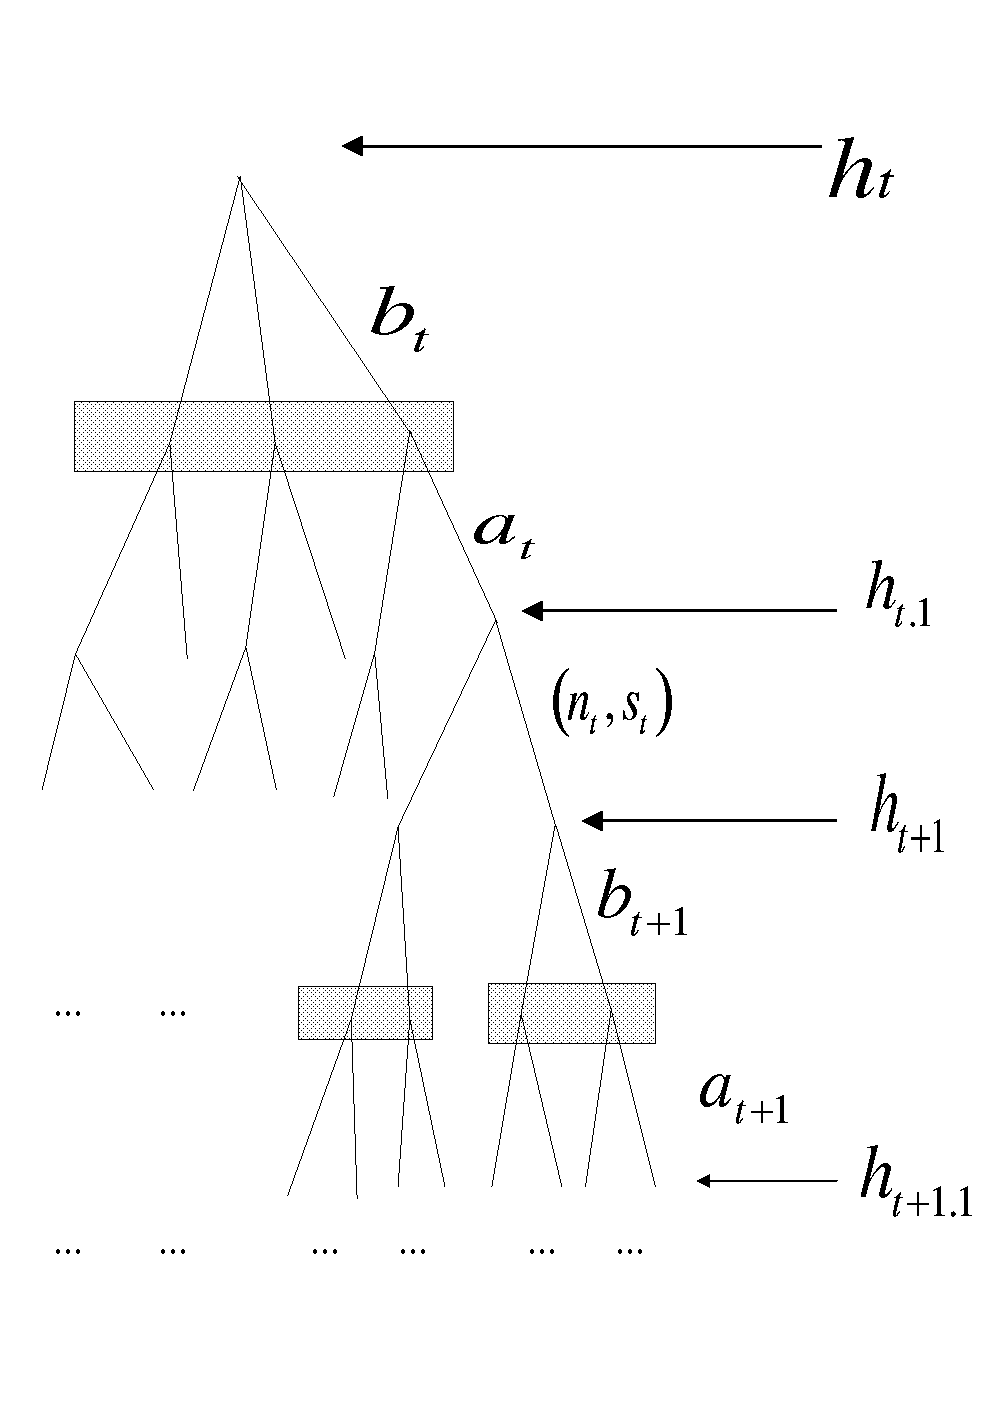
\includegraphics[height=3.0in,keepaspectratio=true]{tree1.png}
\end{center}
\caption{Extensive form representation of the multi-stage game, $\Gamma(h_t)$}
\label{fig1}
\end{figure}
\end{verbatim}
 
will produce R markdown picture as follows.
 
\begin{figure}[htbp]
\begin{center}
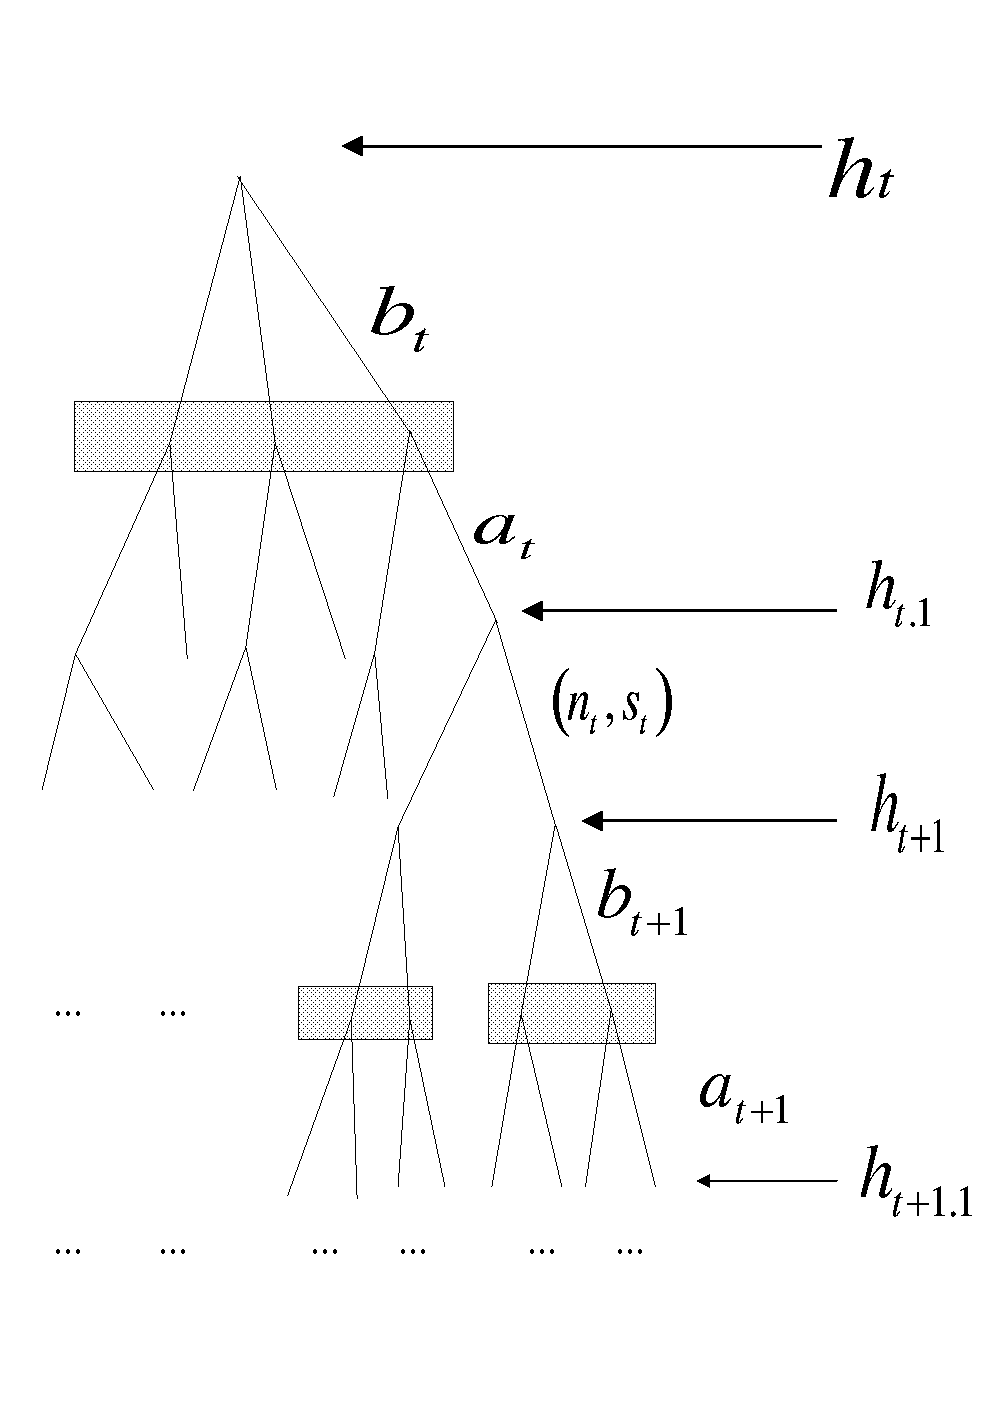
\includegraphics[height=3.0in,keepaspectratio=true]{tree1.png}
\end{center}
\caption{Extensive form representation of the multi-stage game, $\Gamma(h_t)$}
\label{fig1}
\end{figure}

The labeled LaTex figures like the above referred in the Latex text like Figure \verb&\ref{fig1}& ( or, \verb&\autoref{fig1}&) will convert to R markdown document like Figure \ref{fig1} ( or, \autoref{fig1}).

The software can also converts Tikz pictures.  Here is one taken from my \cite{Raut_2017a} paper.

\begin{figure}[tbp]
\begin{tikzpicture}[scale=0.5]
\draw[thick,<->] (0,10) node[left]{$\tau_t$}--(0,0)--(10,0) node[below]{$s_{t-1}$};
\node [below left] at (0,0) {$0$};
\draw(0.5,10) ..controls (1,5) and (3.5,2) .. (10,0.5) node[right]{$\sigma(\tau_t, s_{t-1})=s_t$};
\draw(1,10) ..controls (2,4.5) and (3,3.5) .. (10,1.2) node[right]{$\sigma(\tau_t, s_{t-1})=s'_t$};
\node [below left] at (6,6) {$s'_t > s_t$};
\end{tikzpicture}
\caption{Sets of individuals $(\tau_t,s_{t-1})$ for whom $\sigma(\tau_t,s_{t-1})=s_t$ and $\sigma(\tau _t,s_{t-1})=s^{\prime }_t$}
\label{fig2}
\end{figure}

The following table can be referenced like \verb& Table \ref{table1} or \autoref{table1} & . They render as Table \ref{table1} or \autoref{table1} and link to the same table as you can see.
%==============================================================================
\begin{table}[!h]
\footnotesize\centering
\caption{Steady-state local learning and subgame perfect gift equilibria for the economy with $\delta _{0}=0.35$}
\label{table1}\vspace {.10in}
\par
\begin{tabular}{||c|c|c|l||}
\hline\hline
$\tau $ & $%
\begin{array}{l}
\text{Equilibrium} \\ 
\text{Concept}%
\end{array}
$ & $\sigma ^{\prime *}$ & $\left( n^{*},s^{*},a^{*},U_{\max }\right) $ \\ 
\hline
0 & $%
\begin{array}{l}
\text{Nash} \\ 
\text{Equilibrium}%
\end{array}
$ & - & $%
\begin{array}{l}
(1.699710194,0,.4095616885,-1.140189766) \\ 
(1.025062190,1.341247016,.3341720874,-1.241803182)%
\end{array}
$ \\ \hline
- & $%
\begin{array}{l}
\text{Social} \\ 
\text{Optimum}%
\end{array}
$ & - & $n^{*}=4.4273139,$ $\tau ^{*}=.296681,$ $U_{\max }=-1.066475$ \\ 
\hline
0 & $%
\begin{array}{l}
\text{Fixed} \\ 
\text{Convention}%
\end{array}
$ & 573.2 & $(1.6958508998,0,0.409831247,-1.140547454)$ \\ \hline
0 & $%
\begin{array}{l}
\text{Fixed} \\ 
\text{Convention}%
\end{array}
$ & 0 & $%
\begin{array}{l}
(1.5989049725, 0, 0.41682122123, -1.1501342368) \\ 
(.8658794251, 1.477940857, .3265849827,-1.270158580)%
\end{array}
$ \\ \hline
0 & $%
\begin{array}{l}
\text{Learned} \\ 
\text{Convention}%
\end{array}
$ & -0.121472602158 & (1.59835683672,0, 0.4168619874, -1.1501919166) \\ 
\hline
0.035 & $%
\begin{array}{l}
\text{Learned} \\ 
\text{Convention}%
\end{array}
$ & -0.0884944056 & (1.4123165415, 0, 0.39660878 -1.1724263009) \\ 
\hline\hline
\end{tabular}
\vspace{0.25in}
\end{table}
%=================================================================

\section{List environments: itemize, enumerate, description}\label{sec6}

Enumerate items

\begin{enumerate}
\item One
\item Two
\item Three
\end{enumerate}

Description items

\begin{description} 
  \item Can convert theorems and theorem like environments like proposition, lemma etc.

  \item Can convert proof environment. 
  
  \item Can convert assumption and remark environments: Assumption is user created environment, and remarks either as Latex environment or user created latex environment.
   
  \item Figures: Can convert includegraphics with png files and embedded Tikz figure environment. 
  
  \item Tables: It converts tables as a Rmarkdown table chunk keeping only the label and caption of the Latex tables. The references to the table is also converted throughout the document.  The content of a Latex table may involve complex structure and often created using excel or R and better left for various R packages to create those Rmarkdown table contents in the converted Rmarkdown document.
  
  \item It converts other Latex envirnments: quote, verbatim. I have incorporated Latex commands:  \\section, \\subsection, \\subsubsection,  \\emph, \\texbf \\url \\footnote \\verb.  This document contains all these, so you can compare the source file and converted file to see those.  For other examples, go to my publications page \url{https://lakshmiraut.github.io/publication/}, click on the preprint button, or to my main page, \url{https://lakshmiraut.github.io}.
  
\end{description} 

\section{Theorem like environments} \label{sec7}
I illustrate the content of this section taking a section of my paper, \cite{Raut_2017a}. This involves definition, theorem and proof environments.  Similarly, it will convert other theorem and theorem like environments of your Latex document.
 
\begin{definition}
\label{def1} Initial distribution $\pi ^{0}$ of social groups in $\mathcal{S}$, is given. A \textbf{signaling equilibrium}\index{Signaling equilibrium} is a sequence of probability distributions $\left\{ q_{t}\left( e_{t}|s_{t}\right) \right\} _{1}^{\infty }$ and a sequence of optimal schooling decision rules $\left\{ \sigma _{t}\left( \tau _{t},s_{t-1}\right) \right\} _{1}^{\infty }$ such that at each period $t\geq 1,$

\begin{enumerate}
\item The induced wage schedule $w_{t}\left( s_t\right) =\int e_{t}q_{t}\left(
e_{t}|s_{t}\right)  de_{t}$ is a smooth concave function.

\item Given $w_{t}\left( s_t\right)$, the function $\sigma _{t}\left(\tau
_{t},s_{t-1}\right)$ solves the schooling decision problem of each
agent $\left( \tau _{t},s_{t-1}\right)$.

\item The induced  conditional distribution $\hat{q}_{t}\left( e_{t}|s_{t}\right)$ of $e_{t}$ given the optimal solution 
$s_{t}=\sigma _{t}\left( \tau _{t},s_{t-1}\right)$ obtained by using Bayes
rule coincides with the anticipated conditional distribution $q_{t}\left(
e_{t}|s_{t}\right)$ for all $s_{t}$.
\end{enumerate}
\end{definition}


I assume the following:

\begin{assumption}
\label{A1}$\theta _{t}(s_{t},\tau _{t},s_{t-1})$ $=\theta _{1}\left( s_{t}\right) \cdot \theta _{2}\left( \tau _{t}\right) \cdot \theta _{3}\left( s_{t-1}\right) ,$ $\theta _{1}\left( {}\right)$ is smooth, monotonically increasing and concave, $\theta _{2}\left( {}\right)$ and $\theta _{3}\left( .\right)$ are smooth, monotonically decreasing.
\end{assumption}

\begin{assumption}
\label{A2}The distributions $g\left( \tau \right)$ and $\pi _{0}\left( s_{0}\right)$ belong to a concave conjugate family.
\end{assumption}

\begin{theorem}
Under \autoref{A1} and \autoref{A2}, there exists a signaling equilibrium.
\end{theorem}

\begin{proof}
Suppose we have found a smooth concave wage schedule $w_{t}\left( s\right)$
with a first derivative $w_{t}^{\prime }\left( {}\right)$. The first order
condition of the optimization problem is given by 

\begin{equation}
 \frac{w_{t}^{\prime }\left( s_{t}\right) }{\theta _{1}^{\prime }\left( s_{t}\right) }=
 \theta _{2}\left( \tau _{t}\right) \theta _{3}\left( s_{t-1}\right) \label{eq10}
\end{equation}

The rest is given in \cite{Raut_2017a}.

\end{proof}

\section{Remarks} \label{sec8}

A latex document may have numbered  remarks and later referred those remarks by their numbers.  To enable this I use a special construct so that remarks are numbered and and can have labels which can be used to refer to them in the text.


\begin{remark}
The processing of Rmarkdown file is best done in Rstudio. It can also be done in R. You need to have the following R packages in R or Rstudio, issuing command: install.packages(c("knitr","rmarkdown","bookdown","reticulate","pdftools","magick")). Package reticulate is needed if you want to incorporate python codes in Rmarkdown document. Apart from R, you need to have a Latex document processing system such as Miktex for windows and Tex Live for Linux.  You also need pandoc which is automatically installed with RStudio installation, otherwise you need this package. You also need to pandoc's pandoc-crossref package that can work with your pandoc package.  
\end{remark}


\begin{remark}
\label{re10}This remark can be referred in the text. In the latex document using its convention. 
To see how it is to be done in Rmarkdown, see the converted Rmarkdown document and the text below it.
\end{remark}

The LaTex code for the above remark is
\begin{verbatim}
\begin{remark}
\label{re10}This remark can be referred in the text. In the latex document 
using its convention. To see how it is to be done in Rmarkdown, 
see the converted Rmarkdown document and the text below it.
\end{remark}
\end{verbatim}
Let me point out that the reference to a remark with a label for instance in the above LaTex code will be converted. 
For instance LaTex code Remark \verb&\ref{re10}& or \verb&\autoref{re10}&) will refer to Remark \ref{re10} or \autoref{re10} in the converted document. Unfortunately, the reference is not clickable to go to the remark at this time.

\section{Footnotes} \label{sec9}
The footnotes with latex math often results in nested curly brackets. This is also taken care of automatically.  For instance text like,

\begin{verbatim}
This is a note\footnote{I have used $x^2$ and $x_{10}$ which involve curly brackets 
within the footnote.} and the test continues. Another note\footnote{
this one involves deeper nested curly braces $\frac{x^{2}}{y^2}$ in the footnote.}. 
Both should convert properly.
\end{verbatim}

This is a note\footnote{I have used $x^2$ and $x_{10}$ which involve curly brackets 
within the footnote.} and the test continues. Another note\footnote{
this one involves deeper nested curly braces $\frac{x^{2}}{y^2}$ in the footnote.}. 
Both should convert properly.

\printbibliography
\end{document}